\chapter{State of Art and first decisions}

In this chapter, we are going to talk about the state of art in two domains.
On one side we have the analysis of the similar projects or applications that
already exists in the market, which would be the state of art of the problem
that we want to solve and by other side, the technologies that we can choose
to solve this, it would be the state of art to the implementation.

\section{Problem domain}

The developing of a new complete system have no sense if before have not been
analyzed other existent solutions. As part of the research process has been
analyzed some applications that (although are not a direct competence) represent
the actual state of the art about the kind of software we are talking about.
\intro
First, we take a look at the main features that are important in our domain
to see how many applications have covered them. These are a few requirements
analysis but not very formal, we will discuss about this after.
\intro
\pagebreak
\intro In the following table, we are going to compare the rest of app with our idyllic
software (with the features we hope it will cover).

\begin{table}[H]
\centering

\begin{tabular}{@{}lllllll@{}}

Feature & classDojo & TeacherKit & A+ & iDoceo & Additio & SMS \\ \midrule
Attendance & \completeValue & \completeValue & \completeValue & \completeValue & \completeValue & \completeValue \\
Discipline & \partialValue & \completeValue & \completeValue & \completeValue & \completeValue & \completeValue \\
Attitude & \partialValue & \completeValue & \completeValue & \completeValue & \completeValue & \completeValue \\
Marks & \noneValue & \completeValue & \completeValue & \completeValue & \completeValue & \completeValue \\
Competencias & \noneValue & \noneValue & \noneValue & \completeValue & \completeValue & \completeValue \\
Rubrics & \noneValue & \noneValue & \noneValue & \completeValue & \completeValue & \completeValue \\
Message & \completeValue & \completeValue & \completeValue & \noneValue & \noneValue &	\completeValue \\
patters & \noneValue & \noneValue & \noneValue & \completeValue & \completeValue & \completeValue \\
reports & \noneValue & \completeValue & \completeValue & \partialValue & \completeValue & \completeValue \\
analysis & \partialValue & \completeValue & \partialValue & \partialValue & \partialValue & \completeValue \\
models and predictions & \noneValue & \noneValue & \noneValue & \noneValue & \noneValue & \completeValue \\
Centralizate and jerarqy & \noneValue & \partialValue & \noneValue & \noneValue & \noneValue & \completeValue \\ \midrule

Total & 58.3\% & 80.5\% & 72.2\% & 	72.2\% & 80.5\% & 99\% \\
\end{tabular}
\caption{Features}
\label{my-label}
\end{table}

\noindent As we can see, there are some apps that are so focused on their specific domain
that is very deficient in the rest. In spite of this are referents in
their area, and their numbers of users are huge (only have been compared apps
that have a good acceptance by users).
\intro
But is not only important the features of the software, because with time and
effort any feature can be added. There are other things in the background that
are really important too and that can be that to grow our app steadily or that crash
when we have thousand of users. We are talking about something as data control,
performance, scalability or centralización (we do not explain in detail each one because
is out of his work but we think is also very important).
And of course, all related to interface and user experience, that in most of
cases can represent the difference between the successful and failure of our
project.
\intro
\pagebreak
\intro
So, based on it this is our comparative:



\begin{table}[H]
\centering

\begin{tabular}{@{}lllllll@{}}

Feature & classDojo & TeacherKit & A+ & iDoceo & Additio & SMS \\ \midrule
Personalization & \noneValue & \noneValue & \noneValue & \noneValue & \noneValue & \noneValue \\
UI & \partialValue & \completeValue & \completeValue & \completeValue & \completeValue & \completeValue \\
UX & \partialValue & \completeValue & \completeValue & \completeValue & \completeValue & \completeValue \\
Price & \noneValue & \completeValue & \completeValue & \completeValue & \completeValue & \completeValue \\
Performance & \noneValue & \noneValue & \noneValue	 & \completeValue & \completeValue & \textcolor{ownGreen}{\completeValue} \\
Scalability & \noneValue & \noneValue & \noneValue & \completeValue & \completeValue & \completeValue \\
Data control & \completeValue & \completeValue & \completeValue & \noneValue & \partialValue & \completeValue \\
Multiplatform & \noneValue & \noneValue & \noneValue & \completeValue & \completeValue & \completeValue \\
Centralization & \noneValue & \completeValue & \completeValue & \partialValue & \completeValue & \completeValue \\ \midrule

Total & 44.4\% & 50.0\% & 16.6\% & 	16.6\% & 44.4\% & 99\% \\
\end{tabular}
\caption{Architecture and design}
\label{my-label}
\end{table}

\noindent Obviously, only in the hypothetical case of our app is fully developed will cover
all the aspects considered, but before of the research is easy to understand that
is not so difficult cover all with the correct design, architecture or design.
\intro
And we are going to try to give a simple and really little approximation of the way
to achieve that.
\intro
So, \textbf{let's start!}


\section{Implementation domain}


Nowadays we can build almost any kind of software with a lot of differents
language from which to choose, but as if that were not enough there
are also a lot of architectures that are possible to follow, and beside
of this it will be necessary choose where to deploy our software, or how
doc it, or how to manage our work team, etc. A lot of options that it
will be necessary to choose and that can make the difference between the
success or failure of our project. So, what about of these decisions
in this project? We are going to take a look at it, tools, patterns and
\textit{we will take some firsts decisions about it.}

\subsection{Architecture}

Almost any kind software or tool can be built of differents ways, independently
of this behavior or the goals that it must achieve. Some ways are more specific
to achieve some specific behavior and other although useful are not the best option.
Because of this, we need this phase of research, to avoid, as far as possible, make mistakes before to start.

\subsubsection{Kind of software}
We can think of a mobile app, but what happens with desktop users? And even if
we do a mobile app, for what operating system? Too options for to develop a solution
for each one. Based on informal requirements was thought that the best option could be a
\textbf{web app} for a lot of reasons. First of all because is the simplest
way to offer an app that can run on almost any device (with a \textit{
simple\footnote{Actually a browser is one of the more complex pieces of
software, but here is labeled as simple because is a software that the
majority of devices like smartphones, tablet, etc, have by default and for
the most nontechnical people isn't a complex software, nothing could be
further from the truth.}} browser). Also because is the easiest way, with the best
learning curve and to end because can be used a lot of different technologies to the same domain.

\subsubsection{Why microservices?}

When we think about an app, of any type, the most of the time we think of a software
running on a single machine, with more or less hardware available, where all
related to the software are inside of the same machine.
\intro
Now, we hearing all the time about microservices, which are in synthesis the
opposite of the traditional monolithic classical approach in software architecture,
and seem like if your design is not based in this mean you are outdated or your design is directly wrong.
Well, this is not totally true but neither false. The goal of this section is
not describe the advantages and drawbacks of this approach, but yes justify why
is their choice.
\intro
Microservices are actually a variant of SOA\footnote{Service-oriented architecture (SOA)
was first described by Gartner in 1996 and is a style of software design where
services are provided to the other components by application components, through
a communication protocol over a network.},that simplify a lot the architecture
of a software system spliting their different systems, doing that work together
to offer the service which the software was design.
Dr. Peter Rodgers introduced the term \textit{"Micro-Web-Services"} during a presentation
at textit{Cloud Computing Expo} in 2005 and as we can see in the following graphic (extracted
using \textit{sotagtrends.com}), the interest of the community about this emerging technology
has never stopped growing.

\begin{figure}[H]
  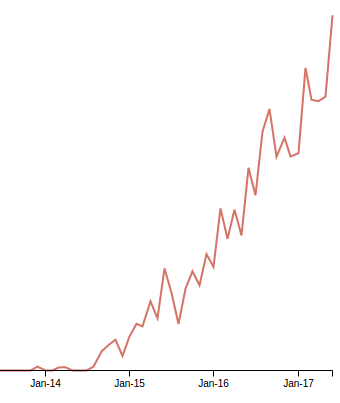
\includegraphics[scale=0.5]{img/graphics/microservices_trend.png}
  \centering
  \caption{Search trend of "microservice" tag in Stack Overflow.}
\end{figure}

\noindent James Lewis\footnote{Principal Consultant at ThoughtWorks and
member of the Technology Advisory Board.} and Martin Fowler\footnote{Software developer,
author and international public speaker on software development, specializing in
object-oriented analysis and design, UML, patterns, and agile software development
methodologies, including extreme programming.} are the major defensor of this
arquitecture and these brings us to the perfect definition of microservices:
\bigskip

\begin{minipage}{0.9\linewidth}
        \vspace{5pt}
        {\small
        \textit{"In short, the microservice architectural style is an approach to developing a
        single application as a suite of small services, each running in its own process
        and communicating with lightweight mechanisms, often an HTTP resource API.
        These services are built around business capabilities and independently deployable
        by fully automated deployment machinery. There is a bare minimum of centralised management
        of these services, which may be written in different programming languages and
        use different data storage technologies."}
        }
        \begin{flushright}
            (Lewis/Fowler)
        \end{flushright}
        \vspace{5pt}
    \end{minipage}

To know more please see \cite{Fowler14Micro}.
\intro
Language agnostics, scalables, adjustables size, independent. our system design
splited in litle pieces with this boundaries make this architecture perfect for
our goals, and this is why we take this choice.

\subsubsection{Why polyglot database?}

With mircroservices-based approach the system will need differents databases to do
some diferent things. In general we can see our
backend like a black box when the data persists in a polyglot database.
That means that the data is saved in differents ways, using different
formats and diferent drivers to manage this. There are a group of
data that would have need be saved with certain relations, due to its nature
and a relational database seem perfect to do this, but this kind of
databases (like MySQL) can be slowly or too heavy for other tasks
of kind of processes, like data analysis.


\subsection{Storage}

With the storage occurs the same, there is a huge list of options to
choose. The fast answer in the most of the cases is: Why do not use a relational
database, as MySQL for example? If we are thinking in a little system
it could be a good choice, always that our data model is adjusted to this kind of system.
But every people knows the deficits and the complexity of the development of a system
with this database. Mainly the performance when we are talking about million
of arrays of objects stored. So, as we was talking before, our goal in this project
is work with a lot of data, of which some are pure relational and another not,
and can be processed by another way, using another engine and database.
\intro
If you have a logical data model like as this project have is not easy choice one
of all database engine to model this. SQL systems is very powerful for some
things but not for another (or not simply) and object oriented databases is
really powerful and simple to develop with it when the data haven't a lot of
relations (although can be modeled also).
so, why choice one between them? Why do not both? This is the approach selected,
build a system with a Polyglot Database, that means: much better select the better
engine for any kind of data instead of trying to use the same for all.
\intro
And this approach joined with microservices architecture give us the first
Conceptual design of our system, where each microservice have their domain work and their
own data, using for their own database engine, and
Until their own language is it will be required.
\intro
So, focused on this project, we are going to use mainly two systems, SQL
relational database system in a service (we will talk more about it after),
and a NoSQL service, in this case, Google Datastore, a fast and lightweight
engine to mange an object oriented database.
\intro
\\
At the moment to write this chapter had been evaluated MongoDB as the best
choice, but the facilities of the platform selected (detailed after) was made
that the G. Datastore was selected finally. Beside of this if the project are
rebuild now have not doubt, Mongo will be selected after the experience ( the
reasons will be explained in more detail in the conclusion of the work).

\subsection{Code strategy}

Entire project will be stored in a single repository, using git as control
versions system.

\subsubsection{Version Control System}

Git\footnote{Git is a free and open source, distributed version control system
created by Linus Torvalds.} is the perfect tool to achieve maintain a more o
less easy workflow between developers minimizing the risks, and the huge list of
plugins to different software and IDEs do this perfect to work, dismissing another
as Subversion, Mercurial, Fossil, or Bazzar.
\intro
The reason to use a single repository is that the mechanism to maintain the
consistency between projects is not easily enough to do the develop agile.
In spite of, git offers us a lot of tools that can improve enormously our
workflow, as the Git Submodules\footnote{Submodules allow you to keep a
Git repository as a subdirectory of another Git repository.
This lets you clone another repository into your project and keep your commits
separate.}, or Git Hooks\footnote{Git has a way to fire off custom scripts when
certain important actions occur. There are two groups of these hooks:
client-side and server-side. Client-side hooks are triggered by operations such
as committing and merging, while server-side hooks run on network operations
such as receiving pushed commits.} between another.

\subsubsection{Hub}

For another hand we have to do another choice, select the remote hub of our repositories
or Git repository hosting service. The most popular for some years has been GitHub,
are a web-based Git or version control repository and Internet hosting service.
It offers all of the distributed version control and source code management (SCM)
the functionality of Git as well as adding its own features,
launched at 2008
but there are other options as Bitbucket\footnote{web-based hosting service
that is owned by Atlassian, used for source code and development projects that
use either Mercurial (since launch) or Git
launched at 2008.},
SourceForge and especially
GitLab\footnote{launched at 2011, was written by Dmitriy Zaporozhets and Valery
Sizov from Ukraine. The code is written in Ruby. Later, some parts have been
rewritten in Go.} (with a big grow ultimately). \pagebreak


\subsubsection{Develop workflow}

Another of the main problem easy to find in the develop when are involved
few people is the organization of the contribution of a repo, but if the project
is composed of few subprojects, this can be worst. For this reason was choose the
strategy to have an only repo with subfolders.
So, took this decision remains to be defined how will work the repo in the
different phases or the develop.
\intro
To do this, we will follow the standard, using branches to develop features and
maintain a good state of the versioning of project.
\intro
So, as we can see in the picture, we are going to use \textit{develop} branch
to do the develop, where we are going to work in minimal changes and will do
a fork when we want to do some representative change in the code, as new functionality or
some big correction.


\begin{figure}[H]
  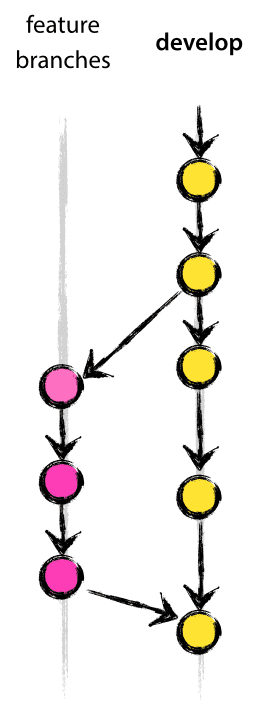
\includegraphics[scale=0.25]{img/git/feature_branches.png}
  \centering
  \caption{Workflow with features branches}
\end{figure}

\noindent For other hand when the all code to launch a final release we will fork the
repo in a \textit{release} branch to while the team continue with the develop
in the mainly develop branch ot in a issue form of this another part of the
team (or itself, is the same), will prepare the code to production, taking a look
because there are some bug, fix it and when all are testend an correctly working
put the project in exactly this verison in master (doing a merte) and this is
when officially a new version of program will be launched.

\begin{figure}[H]
  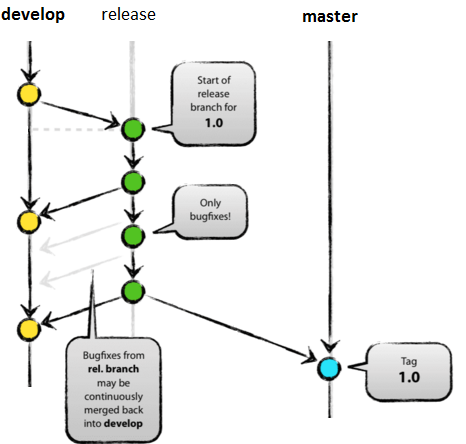
\includegraphics[scale=0.5]{img/git/release_branches.png}
  \centering
  \caption{Workflow with releases branches.}
\end{figure}

\noindent There are some variations of this standard workflow but for this kind of project
is perfect.

\subsection{Languages and frameworks}

As has been said before, almost any kind of software can be built at infinite
ways, and this start with what language can do this. This means it could be
built with Java, Python, C++, Go, Ruby, JavaScript, PHP,  (only talking about
backend) and with another list to the frontend, in this deep list of possibilities,
we choose the most flexible and powerful of all of them, Python and JavaScript.
\intro
Python because is one of the most simplest and powerful languages nowadays, and
JavaScript because is all a standard in the industry. Obviously, the choice is
based also on the fact of both languages are really supported by the community, have a
good learning curve and a lot of projects and systems are based on them.
\intro
JavaScript has been selected because Angular is written in it. AngularJS is the
most powerful framework nowadays to build fast, clean and powerful web apps.
\intro
To exchange data between service we need to select an idiom which the services
will talk, which they will exchange information. That's mean mainly select how
will transform the objects and data structures that services will manage to be able
sender across the net.
\intro
We have some data serialization solutions, some very popular and another most
specific of very focused domains. So, the most commons are JSON, YAML,
BSON and ultimately MessagePack. Each one has their owns benefits and drawbacks but
the selection has been easy, JSON.
\intro
\textbf{XML}
\intro
Extensible Markup Language, is a markup language, defined v1.0 by
W3C\footnote{World Wide Web Consortium, founder by Tim Berners-Lee at 1994 at MIT
(Massachusetts Institute of Technology) the consortium is made up of member
organizations which maintain full-time staff for the purpose of working together
in the development of standards for the World Wide Web.} This is an example:

\begin{lstlisting}[language=xml,frame=none,numbers=none]
  <exam>
    <result>5.8</result>
    <type>Partial</type>
    <subject>Science</subject>
    <date>17-06-2018</date>
  </exam>
\end{lstlisting}


\noindent \textbf{JSON}
\intro
JavaScript Object Notation, is an open-standard file format that uses
human-readable text to transmit data objects based of attribute–value pairs.
Douglas Crockford originally specified the JSON format in the early 2000s
two competing standards, RFC\footnote{ Request for Comments, is a type of
publication from the Internet Engineering Task Force (IETF) and the Internet
Society (ISOC), the principal technical development and standards-setting bodies
for the Internet. were invented by Steve Crocker in 1969 to help record
unofficial notes on the development of ARPANET.} 7159 and ECMA\footnote{Ecma is a
standards organization for information and communication systems founded in 1961
to standardize computer systems in Europe.}-404, defined it in 2013.
The ECMA standard describes only the allowed syntax, whereas the RFC covers some
 security and interoperability considerations.
\intro
In spite of exists a restricted version of JSON, known as I-JSON (short for "Internet JSON"),
defined in RFC 7493, is not as popular as original.
\\This is an example:

\begin{lstlisting}[frame=none,numbers=none]
  {
    "title": "The Picture of Dorian Gray",
    "author": "Oscar Wilde",
    "date": "July 1890"
  }
\end{lstlisting}


\noindent \textbf{YAML}
\intro
Is other Markup Language, commonly used for configuration files but that can
be used in transmision also. Actually is a superset of JSON, whitch latest release
1.2 was published in 2009 and was first proposed by Clark Evans in 2001.
This is an example:

\begin{lstlisting}[frame=none,numbers=none]
  ---
  martin:
      name: Martin D'vloper
      job: Developer
      skill: Elite
\end{lstlisting}


\noindent \textbf{BSON}
\intro
Binary JSON, is a computer data interchange format used mainly as a data storage
and network transfer format in the MongoDB database.
MongoDB represents JSON documents in binary-encoded format called BSON behind
the scenes. BSON extends the JSON model to provide additional data types,
ordered fields, and to be efficient for encoding and decoding within different languages.
\intro
\noindent \textbf{MessagePack}
\intro
Byte array is an efficient binary serialization format, like JSON but faster and smaller and this is an example:

\begin{lstlisting}[frame=none,numbers=none]
{"compact": true, "schema": 0}
27Bytes

82 A7 compact C3 A6 schema 00
18bytes
\end{lstlisting}

\noindent This has several properties really interesting to change in the future
our architecture if will be precise by performance problems (almost all related to internal communications).
See this, \cite{comparision}, interesting benchmark about it.

\subsubsection{Protocol}

Microservices must talk and can do this by differents ways. So, we are going to
take a look over more interesting for us.
\intro
The first that we are talking about is \textbf{REST}. Representational state transfer or
RESTful Web services are one way of providing interoperability between computer systems on the Internet. REST-compliant
Web services allow requesting systems to access and manipulate textual representations
of Web resources using a uniform and predefined set of stateless operations. Other
forms of Web service exist, which expose their own arbitrary sets of operations such as
WSDL and SOAP
\intro
On other hand we have \textbf{RPC}. In distributed computing, a remote procedure call  is when a computer program
causes a procedure (subroutine) to execute in another address space (commonly on
çanother computer on a shared network), which is coded as if it were a normal (local)
procedure call, without the programmer explicitly coding the details for the remote interaction.
\intro
And finally \textbf{gRPC} . It is an open source remote procedure call (RPC) system initially developed at
Google. It uses HTTP/2 for transport and provides features such as authentication, bidirectional streaming and
flow control.
It generates cross-platform client and server bindings for many languages.
We will talk a bit more about this in the Develop chapter.


\subsubsection{Testing}

The tool that we will use for any testing involved in the backend of the project
will be PyTest. Launched at 2004 by Holger Krenel is one of the most complete
suites for testing over Python.
Is really easy to use and allow do some things that is very difficult with another
frameworks as built-in \textit{unittest} python package, somethings as the use of
fixtures of or the amount of plugint that it has.
\intro
Focused on the problem it will be used to make all unittest of the core of services,
libraries and auxiliary programs and testing the entire functionality of the service
when it has a role of black box.


\subsubsection{Documentation}

As is saided the tool Sphinx is used to build the doc of the service.
That basically inspect the code files mixing this with all the files
that we write (pure doc) to show this as a web based documetnation
(easy to read and understand).


\subsection{Platforms}

Today, with the explosion of the cloud is necessary a lot of infrastructures that support
All that all companies that want to migrate their businesses model to cloud need.
This is possible thanks to the companies that offer solutions to this, and another that after
Was introduced to the same businesses offering software and hybrid solutions.
Actually, there are a lot of companies that offer some solutions to software (not necessary)
Companies to work with the cloud to build cloud-based solutions and cloud computing easily.
\intro
There are a lot of companies and solutions but only a few are relevant in this domain.
Although the classifications always can change there are three kinds of service
where each solution can be classified.
\intro
The first is \textbf{IaaS} (Infrastructure as a Service), that means the pure
infrastructure, only servers, virtual machines in cloud data centers with some
 management tools in the majority of the cases where all internal management of
 this machines is work of the customer. Examples of these are
Amazon Web Service, Google Computer Engine, Rackspace Cloud or vCloud.
The second is
\intro
\textbf{PaaS} (Platform as a Service), where above of infrastructure was implemented
services that abstract the management of the \textit{"metal"}. Normally services
where the developers build the code and run this in some services. An example of more
common is Google App Engine or Heroku.
\intro
The last one is \textbf{SaaS} (Software as a Service), in this case only is offered
software solutions in line, which customers do not need worry about updates,
installation or somethings like this. An example of this is famous Google Docs,
Salesforce, Dropbox or the traditional email managers as Gmail. Almost any online
service can be framed here.
Let's take a look to more important nowadays.
\intro
\textbf{Amazon Web Services}
\intro
Launched at 2006 The most popular include Amazon Elastic
Compute Cloud (EC2) and Amazon Simple Storage Service (S3).
\intro
\textbf{Microsoft Azure}
\intro
Is a cloud computing service created by Microsoft for building, testing, deploying,
and managing applications and services through a global network of Microsoft-managed
data centers. It provides software as a service (SaaS), platform as a service and
infrastructure as a service and supports many different programming languages,
tools and frameworks, including both Microsoft-specific and third-party software and systems.
Azure was announced in  2008 and released in 2010 as Windows Azure,
before being renamed to Microsoft Azure in 2014.
\pagebreak
\intro
\textbf{IBM BlueMix}
\intro
A PaaS developed by \textit{IBM}. It supports a lot of languages and services. It is
based on \textit{Cloud Foundry} open technology and runs on
\textit{SoftLayer\footnote{A dedicated server, managed hosting, and cloud
computing provider, founded in 2005 and acquired by IBM in 2013.}} infrastructure.
\intro
\textbf{Heroku}
\intro
Another PaaS, founded by James Lindenbaum in 2007 at
San Francisco, California,is used as a web application deployment model.
It was acquired by Salesforce.com in 2010.
\intro
\textbf{CloudFoundry}
\intro Is an open source PAAS governed by the Cloud Foundry Foundation that
was originally developed by VMware.
\intro
\textbf{Google Cloud Platform}
\intro Is a suite of cloud computing services
that runs on the same infrastructure that Google uses internally for its end-user
products, such as Google Search and YouTube.Alongside a set of management tools,
it provides, a series of modular cloud services including computing, data storage,
data analytics and machine learning.
\intro
\textit{For all those services that offered and by some experience with it in
some previous little project is because was selected.}

\subsection{Documentation}

To do the documentation of the code as in the rest of sections, we have a few options
to choose. So, as the backend is fully developed in Python we are going to use some python
especially documentation framework and in this case Sphinx\footnote{Sphinx is a
simple and powerful Python-based documentation generator.} has been selected.
\intro
For another hand, to the front, especially talking about Javascript with AngularJS
we do not have the need to a doc because the docstrings have been sufficient,
and neither have been found any really good tool as Sphinx for them. \pagebreak

\subsection{License}

In this project, we are going to use GNU General Public License v3 (GPL-3)
to license our code.
There are a lot of licenses available, but it meets all our needs,
this is a little summary of this:

\begin{table}[H]
  \centering
  \begin{tabular}{ l | c | r }
    Can &  Cannot & Must \\
    \hline
    Commercial use    & Sublicense    &  Include original \\
    Modify            & Hold liable   &  State changes \\
    Distribute        &               &  Disclose source \\
    Place warranty    &               &  Include License \\
    Use patent claims &               &  Include Copyright \\
                      &               &  Include Install Instruction \\
  \end{tabular}
  \caption{License characteristics summary.}
\end{table}

\noindent Although this is one of the most famous, there are a lot of open source
licenses. If we want to know how many projects are licensed with which licenses
there are some research about it. As for example, the made by \textit{Black Duck
(blackducksoftware.com)} that looking at more of 9000 forges and repositories have
calculated these use percentages:  \textbf{MIT}\footnote{A permissive free software
license originating at the Massachusetts Institute of Technology (MIT).} (32\%), GNU 2.0 (18\%),
\textbf{Apache}\footnote{A permissive free software license written by the Apache
Software Foundation (ASF).} 2.0 (14\%), GNU 3.0	(7\%) and \textbf{BSD}\footnote{A
family of permissive free software licenses by the Berkeley Software Distribution (BSD),
a Unix-like operating system.} 2.0 (6\%).
